\title{\vspace{-25mm}Sample Return Robot Challenge 2014 \\ Design Proposal}
\author{Team: RPIRR (Rensselaer Polytechnic Institute Rock Raiders)}
\date{\today}
\documentclass{paper}

%% Packages
\usepackage{algorithm}
\usepackage{algorithmicx}
\usepackage{amsfonts}
\usepackage{amsmath}
\usepackage{bm}
\usepackage[labelfont=bf]{caption}
\usepackage{colortbl}
\usepackage{graphics}
\usepackage{graphicx}
\usepackage[ 	colorlinks = true,
            		linkcolor = blue,
            		urlcolor  = blue,
            		citecolor = blue,
           		anchorcolor = blue]{hyperref}
\usepackage{pifont}
\usepackage{setspace}
\usepackage{sidecap}
\usepackage{subcaption}
\usepackage{tikz}
\usetikzlibrary{arrows,fadings,positioning,shapes,snakes}
\usepackage{titlesec}
\usepackage{url}
\usepackage{wrapfig}
\usepackage{xcolor}



%% Useful commands
\newcommand{\tab}{\hspace*{2em}}
\newcommand \todo[1]{\textcolor{red}{[#1]}}
\newcommand \robotName{Rockie} 		% Edit here to change robot name


%%%%%%%%%%%%%%%%%%%%%%%%%%%%%%%%%%%%%%%%%%%%%%%%%%
\begin{document}
\maketitle


%%%%%%%%%%%%%%%%%%
% Overview
\section*{Overview of design}

	This document contains a brief overview of our design goals as well as relevant descriptions of materials and preliminary design choices.  As this is our first year participating, we will be trying to keep our design straight forward.  ``\robotName" will be a four-wheeled mobile robot with 1-DOF mandibles.  Objects will all be stored in the hull, separated by cloth or plastic dividers.   An on board computer running ROS will control the autonomous sensing, roving, and object acquisition.   
%attached to a 3-DOF arm, bins for separating retrieved objects, multiple cameras, and autonomous controls built in ROS.  

\begin{figure}[h]
\centering
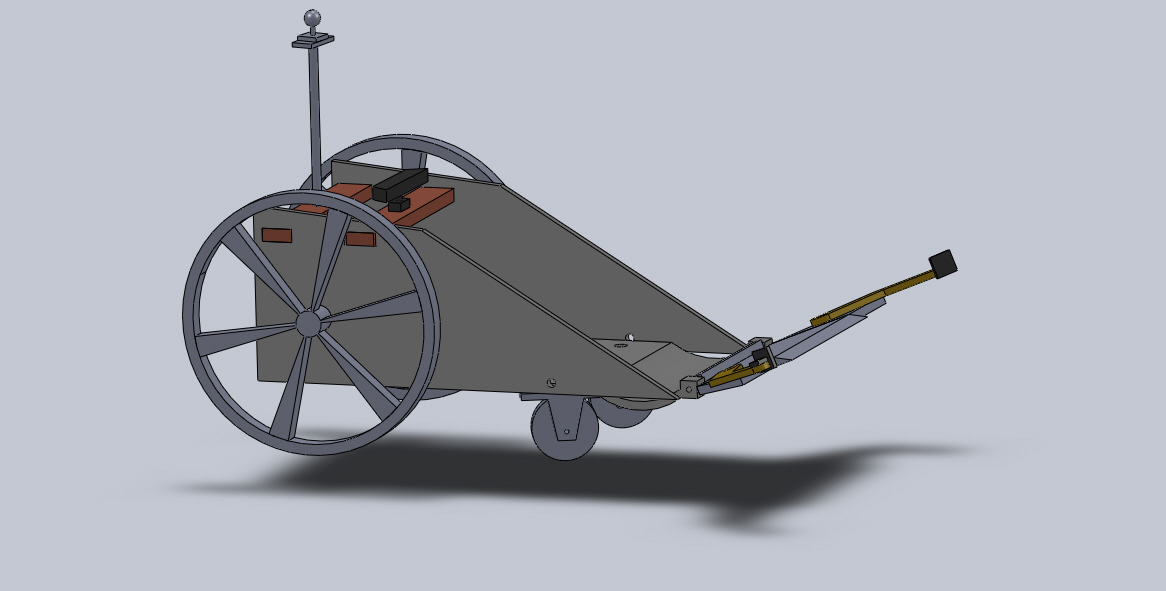
\includegraphics[width=0.65\textwidth]{fig/robot_assemble_scoop.JPG} \\ 
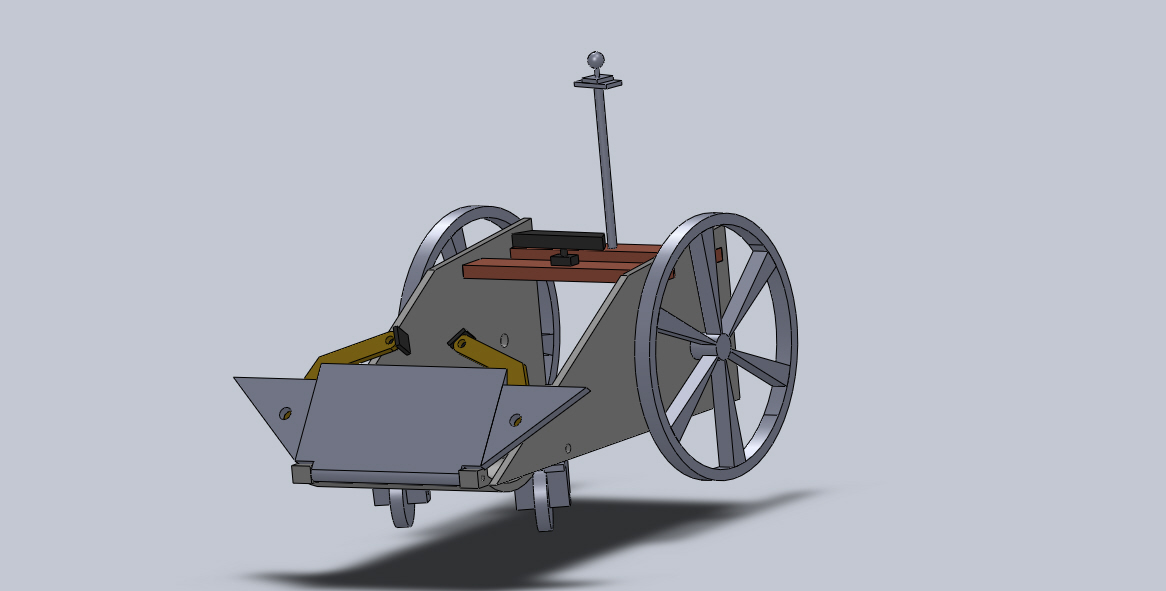
\includegraphics[width=0.65\textwidth]{fig/robot_assemble_scoop_2.JPG} \\
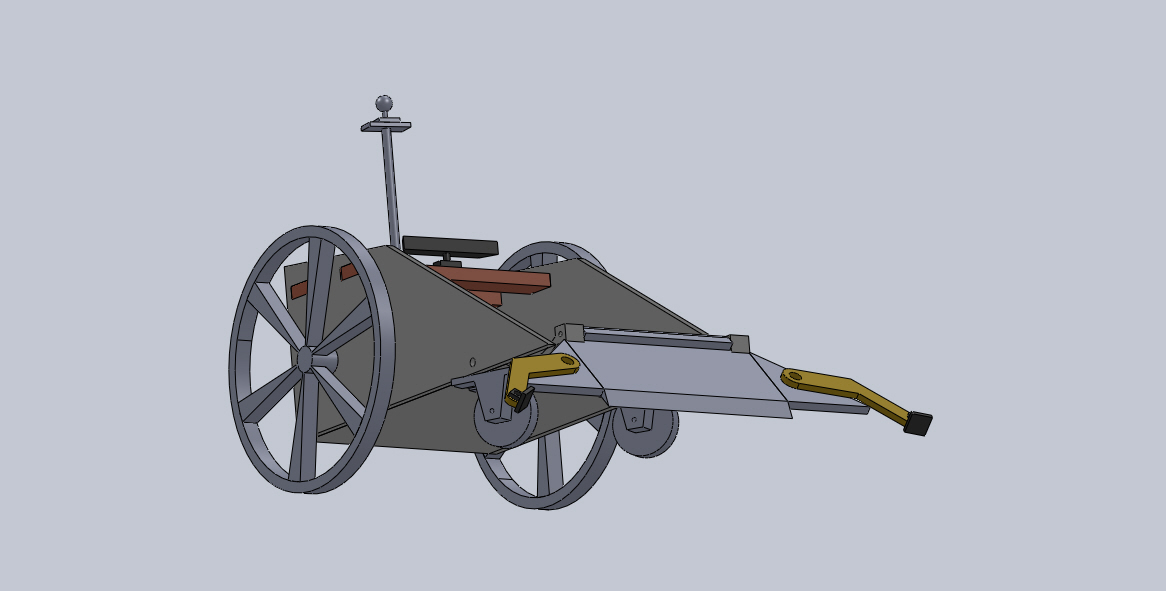
\includegraphics[width=0.65\textwidth]{fig/robot_assemble_scoop_4.JPG}
\caption{A sketchup of \robotName. }
\label{fig:sketchup}
\end{figure}

%%%%%%%%%%%
\subsection*{Hardware and electronics}

	% Communication protocols and frequencies used.
	The only communication we anticipate implementing is a wireless pause switch.  For this, we will use an XBee PRO at 2.4 GHz, since it has excellent range and is easy to use.

	% Sensors for localization, navigation, obstacle avoidance, and sample id
	\robotName\text{ }will be equipped with at least two cameras: 
\begin{itemize}
	\item A high-definition color camera for long range perception (mounted on the pole in Figure~\ref{fig:sketchup})
	\item A Kinect for point cloud data and SLAM refinement at medium range
	%\item A low-definition camera mounted near the gripper for use during grasping.
\end{itemize}
All cameras will be able to contribute to object and sample identification.  
	Navigation, including localization and obstacle avoidance, will involve the very popular SLAM approach.  In particular, we will utilize the rgbdslam ROS package.  


%%%%%%%%%%%
% Electronics
	The following is a list of electronic components we will use in addition to the cameras:
\begin{itemize}
	\item Laptop running ROS
	\item 2x geared 12V DC motor with H bridges
	\item Arduino as motor controller
	\item Deep-cycle lead-acid battery and voltage regulator
	\item High torque servo or small DC motor for mandibles 
\end{itemize}
We are currently deciding between methods of how to store acquired objects without contamination.  Our approach will likely involve scooping the object onto the front of the hull onto sheets of plastic.  Each sheet can be drawn up or folded over to make contain it and make room for the next object.  



%%%%%%%%%%%
\subsection*{Safety features}

	% Wireless kill switch / on-board E-Stop
	\robotName \ will have a master power switch, mechanical e-stop, and wireless pause switch in accordance with rules R18 and R19.  \robotName \ will also have a safety light to display its state.  Currently, we do not plan to provide power to the home beacon.  
	% Hazardous materials compliance (battery?)
	\robotName \ will contain no hazardous materials as per rule R17.  



%%%%%%%%%%%
\subsection*{Software}

	We will use ROS as our software platform since it offers many useful libraries, in particular SLAM, SIFT, and PCL to name a few.     





\end{document}



























